\setcounter{section}{0}

\section{Lecture 1: Introduction, Degrees of Freedom, and Lagrangian Dynamics}

\subsection{Introduction}

The objective of this course is to develop a deep understanding of classical dynamical systems through the lens of Lagrangian mechanics. We will explore how systems evolve over time by transitioning from Newtonian formulations to a more elegant and generalized Lagrangian framework.

\subsubsection*{Coordinate Systems}

\paragraph{Cartesian Coordinates.}
In Cartesian coordinates, the position, velocity, and acceleration of a particle are given by:
\begin{equation}
    \begin{aligned}
        \mathbf{r} & = (x, y, z)         \\
        \mathbf{v} & = \dot{\mathbf{r}}  \\
        \mathbf{a} & = \ddot{\mathbf{r}}
    \end{aligned}
\end{equation}

\paragraph{Polar Coordinates.}
For a planar motion described in polar coordinates $(r,\theta)$, the time derivatives of the unit vectors are:
\begin{equation}
    \begin{aligned}
        \frac{d\hat{\mathbf{e}}_r}{dt}      & = \dot{\theta}\,\hat{\mathbf{e}}_\theta \\
        \frac{d\hat{\mathbf{e}}_\theta}{dt} & = -\dot{\theta}\,\hat{\mathbf{e}}_r
    \end{aligned}
\end{equation}
The position and velocity in polar coordinates become:
\begin{equation}
    \begin{aligned}
        \mathbf{r} & = (r, \theta) \\
        \mathbf{v} & = \dot{\mathbf{r}} = \frac{d}{dt}\Bigl(r\,\hat{\mathbf{e}}_r\Bigr)
        = \dot{r}\,\hat{\mathbf{e}}_r + r\,\dot{\theta}\,\hat{\mathbf{e}}_\theta \\
        \mathbf{a} & = \ddot{\mathbf{r}}
    \end{aligned}
\end{equation}

\paragraph{Three-Dimensional Space.}
For a single particle moving in three-dimensional space, its state is described as:
\begin{equation}
    \begin{aligned}
        \mathbf{r} & = (x_1, x_2, x_3)   \\
        \mathbf{v} & = \dot{\mathbf{r}}  \\
        \mathbf{a} & = \ddot{\mathbf{r}}
    \end{aligned}
\end{equation}

\paragraph{Spherical Coordinates.}
In spherical coordinates, where the position is expressed as $(r,\theta,\phi)$, the velocity is given by:
\begin{equation}
    \begin{aligned}
        \mathbf{r} & = (r,\theta,\phi) \\
        \mathbf{v} & = \dot{\mathbf{r}} = \dot{r}\,\hat{\mathbf{r}} + r\,\dot{\theta}\,\hat{\boldsymbol{\theta}} + r\,\dot{\phi}\,\sin\theta\,\hat{\boldsymbol{\phi}}
    \end{aligned}
\end{equation}

\subsection{Degrees of Freedom and Generalized Coordinates}

Newton's second law, $\mathbf{F} = m\mathbf{a}$, governs the dynamics of a particle. However, when dealing with complex systems—especially those subject to constraints—Newtonian mechanics may become unwieldy. Lagrangian mechanics provides an efficient and systematic approach by using \emph{generalized coordinates}.

\begin{definition}[Generalized Coordinates]
    Generalized coordinates are a set of parameters used to represent the state of a system in a configuration space.  If the coordinates are independent of one another, the number of independent generalized coordinates is defined by the number of degrees of freedom of the system.
\end{definition}

\begin{definition}[Degrees of Freedom]
    The degrees of freedom (DOF) of a system refer to the number of independent parameters required to specify its configuration.
\end{definition}

For a system of $M$ particles in three-dimensional space, without constraints, each particle has 3 degrees of freedom, giving a total of $3M$. When $N$ independent constraints are present, the effective number of degrees of freedom is reduced to:
\begin{equation}
    \text{DOF} = 3M - N.
\end{equation}

\subsubsection*{Examples of Constrained Systems}

In figure \ref{fig:1-1-1}, we have:

\begin{itemize}
    \item \textbf{Two particles connected by a rod:}
          The distance between the two particles is fixed, hence:
          \begin{equation}
              \text{DOF} = 3 \times 2 - 1 = 5.
          \end{equation}

    \item \textbf{Four particles connected by rods with fixed angles:}
          With three constraints due to fixed lengths and an additional three constraints from fixed angles, the system reduces to the degrees of freedom of a rigid body:
          \begin{equation}
              \text{DOF} = 3 \times 4 - 3 \text{ (length constraints)} - 3 \text{ (angular constraints)}
              = 6,
          \end{equation}
          which corresponds to 3 translational and 3 rotational degrees of freedom.

    \item \textbf{Three particles connected by rods with one unfixed angle:}
          Removing one constraint results in:
          \begin{equation}
              \text{DOF} = 3 \times 3 - 2 = 7.
          \end{equation}
\end{itemize}

\begin{figure}[ht]
    \centering
    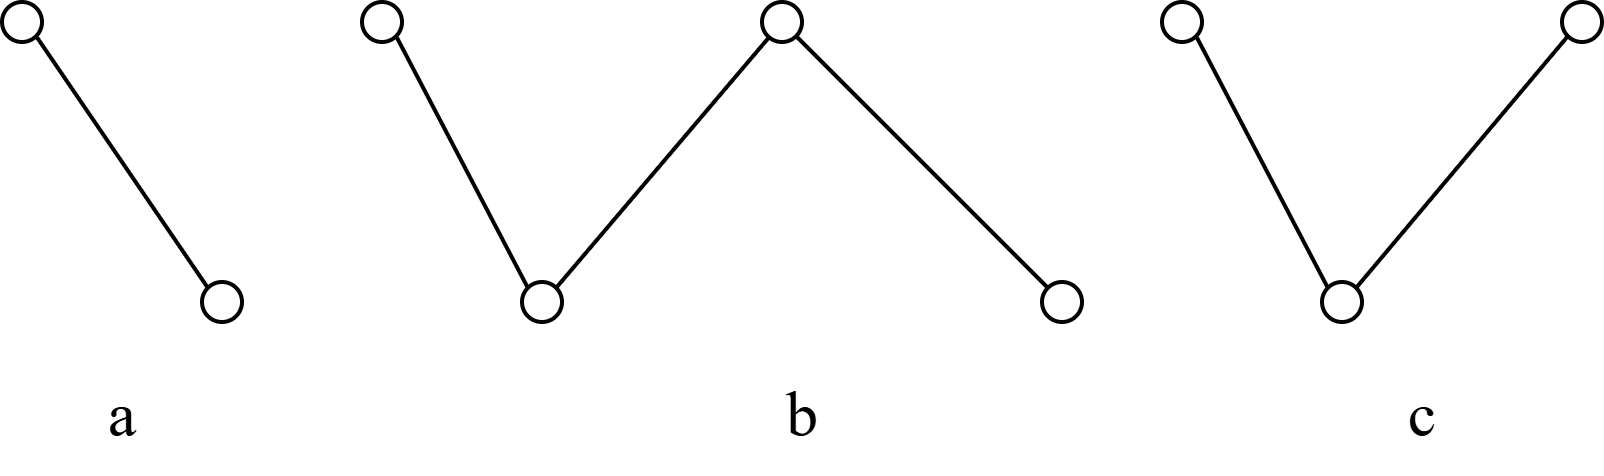
\includegraphics[width=0.8\textwidth]{images/1-1-1.png}
    \caption{Examples of Constrained Systems}
    \label{fig:1-1-1}
\end{figure}

\subsubsection*{The Simple Pendulum}

Consider the simple pendulum depicted in Figure~\ref{fig:1-1-2}. The pendulum's motion is fully described by a single parameter (e.g., the angle $\theta$), hence it has one degree of freedom.

\begin{figure}[ht]
    \centering
    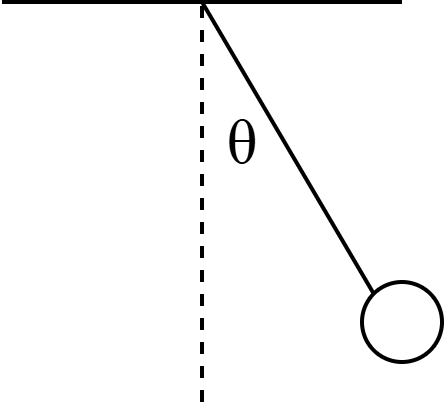
\includegraphics[width=0.3\textwidth]{images/1-1-2.png}
    \caption{Simple Pendulum}
    \label{fig:1-1-2}
\end{figure}

\subsubsection*{Generalized Coordinates for Constrained Systems}

In the context of constrained systems, we introduce a set of generalized coordinates $\{q_i\}$, where $i = 1, 2, \dots, N$, with $N$ being the number of degrees of freedom. The position of each particle in the system can be expressed as:
\begin{equation}
    \mathbf{r}_\alpha = \mathbf{r}_\alpha(q_i, t), \quad \alpha = 1, 2, \dots, M.
\end{equation}
If the equation of constraint contain the time as an explicit variable, then it is referred to as \textbf{rheonomous} constraint; otherwise, it is \textbf{scleronomous}. 

Moreover, if the constraint can be expressed as $f\left(q_1, q_2, \cdots, q_n, t\right)$, where $q_1$, $q_2$, $\cdots$, $q_n$ are the generalized coordinates, without containing velocities and so forth, then it is referred to as \textbf{holonomic} constraint; otherwise, it is \textbf{nonholonomic}.

\begin{figure}[ht]
    \centering
    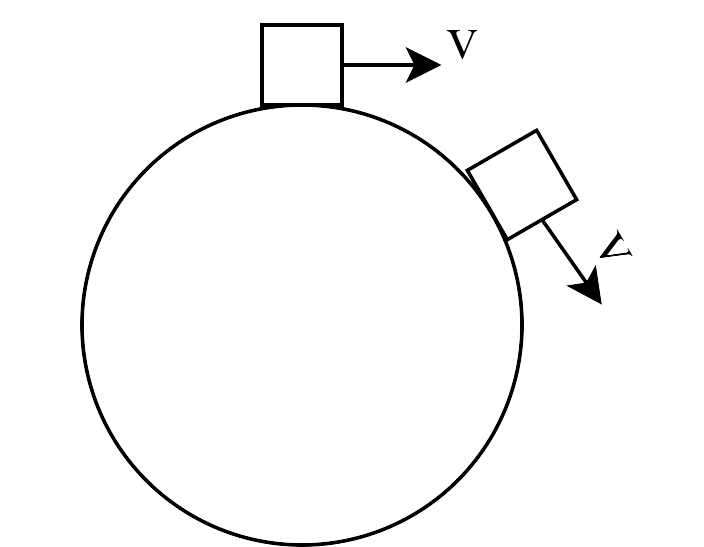
\includegraphics[width=0.3\textwidth]{images/1-1-3.png}
    \caption{Example of a Nonholonomic System}
    \label{fig:1-1-3}
\end{figure}

Nonholonomic systems frequently occur in practice. For example, consider a box moving on the surface of a sphere in figure \ref{fig:1-1-3}: when the box loses contact with the surface, the effective degrees of freedom increase.

\subsection{Lagrangian Mechanics}

Consider a system described by the generalized coordinates $q_i$, where $i = 1, 2, ..., N$ (number of DOF). The positions of the system's parts can be written as $\mathbf{r}_\alpha = \mathbf{r}_\alpha(q_i, t)$. The fundamental problem is to determine the time evolution of these generalized coordinates, $q_i(t)$. These will satisfy a set of $N$ differential equations, known as the \textbf{equations of motion}.

Traditionally, Newton's laws of motion were used, which requires dealing with constraint
forces:

\begin{enumerate}
    \item Determine the force $\mathbf{F}_\alpha$ acting on each part of the system at
          position $\mathbf{r}_\alpha$.
    \item Apply Newton's second law, which gives a system of second-order ordinary
          differential equations (ODEs):

          \begin{equation}
              \mathbf{F}_\alpha = m_\alpha \ddot{\mathbf{r}}_\alpha
          \end{equation}

    \item  Rewrite $\mathbf{r}_\alpha$ in terms of $q_i$. This can be challenging to
          actually implement!
\end{enumerate}

Lagrangian mechanics provides an elegant way to avoid dealing with constraint forces
directly.

Consider an infinitesimal change in position, $\delta \mathbf{r}_\alpha$. The work done
by the force is:

\begin{equation}
    \delta W = \sum_{\alpha} \mathbf{F}_\alpha \cdot \delta \mathbf{r}_\alpha
\end{equation}

A crucial question arises: how much work is done if we change the generalized coordinates
from $q_i$ to $q_i + \delta q_i$? Since $\mathbf{r}_\alpha = \mathbf{r}_\alpha(q_i, t)$,
the variation in position can be written as:

\begin{equation}
    \delta \mathbf{r}_\alpha = \sum_{i} \frac{\partial \mathbf{r}_\alpha}{\partial q_i} \delta q_i
\end{equation}

This assumes that we only consider variations in the generalized coordinates, keeping
$t$ constant. Thus:

\begin{align}
    \delta W & = \sum_{\alpha} \mathbf{F}_\alpha \cdot \left(\sum_{i} \frac{\partial \mathbf{r}_\alpha}{\partial q_i} \delta q_i \right)    \\
             & = \sum_{i} \left(\sum_{\alpha} \mathbf{F}_{\alpha} \cdot \frac{ \partial \mathbf{r}_\alpha}{\partial q_i} \right) \delta q_i
\end{align}

We define the term in the parenthesis to be a \textbf{generalized force}:

\begin{equation}
    F_i = \sum_{\alpha} \mathbf{F}_{\alpha} \cdot \frac{\partial \mathbf{r}_\alpha}{\partial q_i}
\end{equation}

Here, $F_i$ is the generalized force associated with the generalized coordinate $q_i$. It effectively represents the force component in the "allowed" direction defined by the variation in $q_i$.

Now let's consider the kinetic energy of a constrained system:

\begin{align}
    T & = \frac{1}{2} \sum_{\alpha} m_\alpha \dot{\mathbf{r}}_\alpha \cdot \dot{\mathbf{r}}_\alpha \\
      & = T(q_i, \dot{q_i}, t)                                                                     \\
\end{align}

where,

\begin{align}
    \mathbf{r}_\alpha       & = \mathbf{r}_\alpha(q_i, t)                                                                                        \\
    \dot{\mathbf{r}}_\alpha & = \sum_i \frac{\partial \mathbf{r}_\alpha}{\partial q_i} \dot{q_i} + \frac{\partial \mathbf{r}_\alpha}{\partial t}
\end{align}

Note that from the expression above, we have

\begin{equation}
    \frac{\partial \dot{\mathbf{r}}_\alpha}{\partial \dot{q_i}} = \frac{\partial \mathbf{r}_\alpha}{\partial q_i}
\end{equation}

We can compute the partial derivatives of the kinetic energy:

\begin{align}
    \frac {\partial T}{\partial q_i}       & = \sum_\alpha m_\alpha \dot{\mathbf{r}}_\alpha \cdot \frac{\partial \dot{\mathbf{r}}_\alpha}{\partial q_i}                                                                                                            \\
    \frac {\partial T}{\partial \dot{q_i}} & = \sum_\alpha m_\alpha \dot{\mathbf{r}}_\alpha \cdot \frac{\partial \dot{\mathbf{r}}_\alpha}{\partial \dot{q_i}} = \sum_\alpha m_\alpha \dot{\mathbf{r}}_\alpha \cdot \frac{\partial \mathbf{r}_\alpha}{\partial q_i} \\
\end{align}

Now, let's compute the time derivative of $\frac {\partial T}{\partial \dot{q_i}}$:

\begin{align}
    \frac{d}{dt} \left(\frac {\partial T}{\partial \dot{q_i}}\right) & = \sum_\alpha m_\alpha \left(\ddot{\mathbf{r}}_\alpha \cdot \frac{\partial \mathbf{r}_\alpha}{\partial q_i} + \dot{\mathbf{r}}_\alpha \cdot \frac{\partial \dot{\mathbf{r}}_\alpha}{\partial q_i}\right) \\
                                                                     & = \sum_\alpha \mathbf{F}_\alpha \cdot \frac{\partial \mathbf{r}_\alpha}{\partial q_i} + \frac{\partial T}{\partial q_i}                                                                                  \\
                                                                     & = F_i + \frac{\partial T}{\partial q_i}                                                                                                                                                                  \\
\end{align}

Therefore, we have the following important relation:

\begin{equation}
    F_i = \frac{d}{dt} \left(\frac {\partial T}{\partial \dot{q_i}}\right) - \frac{\partial T}{\partial q_i}
\end{equation}

If we know the kinetic energy $T(q_i, \dot{q}_i, t)$, we can obtain the generalized force
without directly calculating constraint forces! This provides a powerful generalization
of $\mathbf{F} = m\mathbf{a}$ to a generic degree of freedom.